\section{Planning in NLG} \label{sec:domains}

In this section, we present our planning domains: the sentence
generation domain and the instruction giving domain.


\subsection{Sentence generation as planning}

Sentence generation is the problem of computing, from a grammar and a
semantic representation, a single sentence that expresses this piece
of meaning.  This problem is traditionally split into several steps
\cite{reiter00building}.  In a first step, called \emph{sentence
  planning}, the semantic representation is first enriched with more
information; for instance, \emph{referring expressions}, which refer
to individuals that we want to talk about, are determined at this
point.  In a second step, called \emph{surface realization}, this
enriched representation is then translated into a natural-language
sentence, using the grammar.

However, determining referring expressions (REs) and realization
interact, so it would be beneficial to perform both steps together.
This was the goal of the SPUD system \cite{Stone2003a}, which
performed both steps together using a top-down generation algorithm
based on tree-adjoining grammars \cite{joshi;etal1997} whose lexical
entries were equipped with semantic and pragmatic information.
Unfortunately, SPUD suffered from having to explore a huge search
space, and had to resort to a non-optimal greedy search strategy to
retain reasonable efficiency.

\cite{KolSto07} attempt to improve the efficiency by translating the
SPUD sentence generation problem into a planning problem and using a
planning algorithm for generation.  We will now illustrate how they do
this by a (simplified) example.

\begin{figure}
  \centering
  xxxx
  \caption{The example grammar.}
  \label{fig:white-rabbit-sleeps-grammar}
\end{figure}

\begin{figure}
  \centering
  xxxx
  \caption{Derivation of ``The white rabbit sleeps.''}
  \label{fig:white-rabbit-sleeps-deriv}
\end{figure}

Consider a knowledge base containing the individuals $r_1$ and $r_2$;
$r_1$ and $r_2$ are rabbits, $r_1$ is white and $r_2$ is brown, and
$r_1$ sleeps.  Let's say we want to express the information
$\{\mathsf{sleep}(r_1)\}$ using the tree-adjoining grammar shown in
Fig.~\ref{fig:white-rabbit-sleeps-grammar}.  This grammar consists of
\emph{elementary trees}, each of which contributes certain
\emph{semantic content}.  We can instantiate these trees by
substituting individuals for \emph{semantic roles}, such as
$\mathsf{self}$ and $\mathsf{subj}$, and then combine the tree
instances as shown in Fig.~\ref{fig:white-rabbit-sleeps-deriv} to
obtain the sentence ``The white rabbit sleeps''.  The SPUD algorithm
computes this grammatical derivation by starting with the elementary
tree for ``sleeps''; this satisfies the need to convey the semantic
information, but introduces a need to generate a noun phrase (NP) for
the subject, which also refers uniquely to the target referent $r_1$.
In a second step, it substitutes the tree for ``the rabbit'' into the
open NP leaf, which makes the derivation grammatically complete; but
as there are two different individuals that could be described as
``the rabbit'' -- technically, $r_2$ is still a \emph{distractor} for
the referring expression --, we are still not finished.  This is why
we add the tree for ``white'' to the derivation by the
\emph{adjunction} operation.  This makes the derivation syntactically
and semantically complete, and we are done.

\begin{figure}
  \centering
  xxxx
  \caption{Generating ``The white rabbit sleeps'' as a planning problem.}
  \label{fig:white-rabbit-as-planning}
\end{figure}

This process has clear parallels to planning: We manipulate a state by
applying actions in order to achieve a goal.  We can make this
connection precise by translating the SPUD problem into a planning
problem; the relevant excerpt of this problem is shown in
Fig.~\ref{fig:white-rabbit-as-planning}.  Each action in this planning
problem corresponds to the addition of a single elementary tree to the
derivation; the first parameter of the action is a node name in the
derivation tree, and the further parameters stand for the individuals
to which the semantic roles will be instantiated.  The syntactic
preconditions and effects are encoded using $\mathsf{open}$ and
$\mathsf{canadjoin}$ literals; the status of each referring expression
is tracked using $\mathsf{distractor}$ literals.  Notice that the
action effects contain terms of the form $\mathsf{subj}(u)$, which
construct new node names.  In order to represent the planning problem
in PDDL, these terms can be eliminated by estimating an upper bound
$n$ for the plan length, making $n$ copies of each action, ensuring
that copy $i$ can only be applied in step $i$, and replacing the term
$\mathsf{subj}(u)$ in an action copy by the constant
$\mathsf{subj}_i$.

In the example, the following plan solves the planning problem:
\begin{enumerate}
\item $\mathsf{sleeps}(\mathsf{root}, r_1)$
\item $\mathsf{rabbit}(\mathsf{subj}(\mathsf{root}), r_1)$
\item $\mathsf{white}(\mathsf{subj}(\mathsf{root}), r_1)$
\end{enumerate}

The grammatical derivation in
Fig.~\ref{fig:white-rabbit-sleeps-deriv}, and therefore the generated
sentence, can be systematically reconstructed from this plan.
Therefore we can solve the sentence generation problem via the detour
through planning and bring current search heuristics for planning to
bear on generation.








\subsection{Planning in instruction giving}

The object of the GIVE Challenge (``Generating Instructions in Virtual
Environments''; Koller et al.\
\citeyear{alexander07:_shared_task_propos}) is to build an NLG system
which is able to give natural-language instructions which will guide a
human user in performing some task in a virtual environment.  A map of
an example world is shown in Fig.~\ref{fig:give-development-world};
instructions for the first steps could be ``turn left; press the
button; turn right and walk through the door;'' and so forth.  From an
NLG perspective, GIVE makes for an interesting challenge because it is
a theory-neutral task that exercises all components of an NLG system,
and emphasizes the study of communication in a (simulated) physical
environment.  It also has the advantage that the user and the NLG
system can be physically in different places, as long as the 3D client
and the NLG system are connected over a network.  This makes it
possible to evaluate GIVE NLG systems on a large scale over the
Internet.  The first GIVE evaluation will take place in late 2008;
currently seven research teams from five countries are working on
developing systems to participate in the challenge.

\begin{figure}
\centering
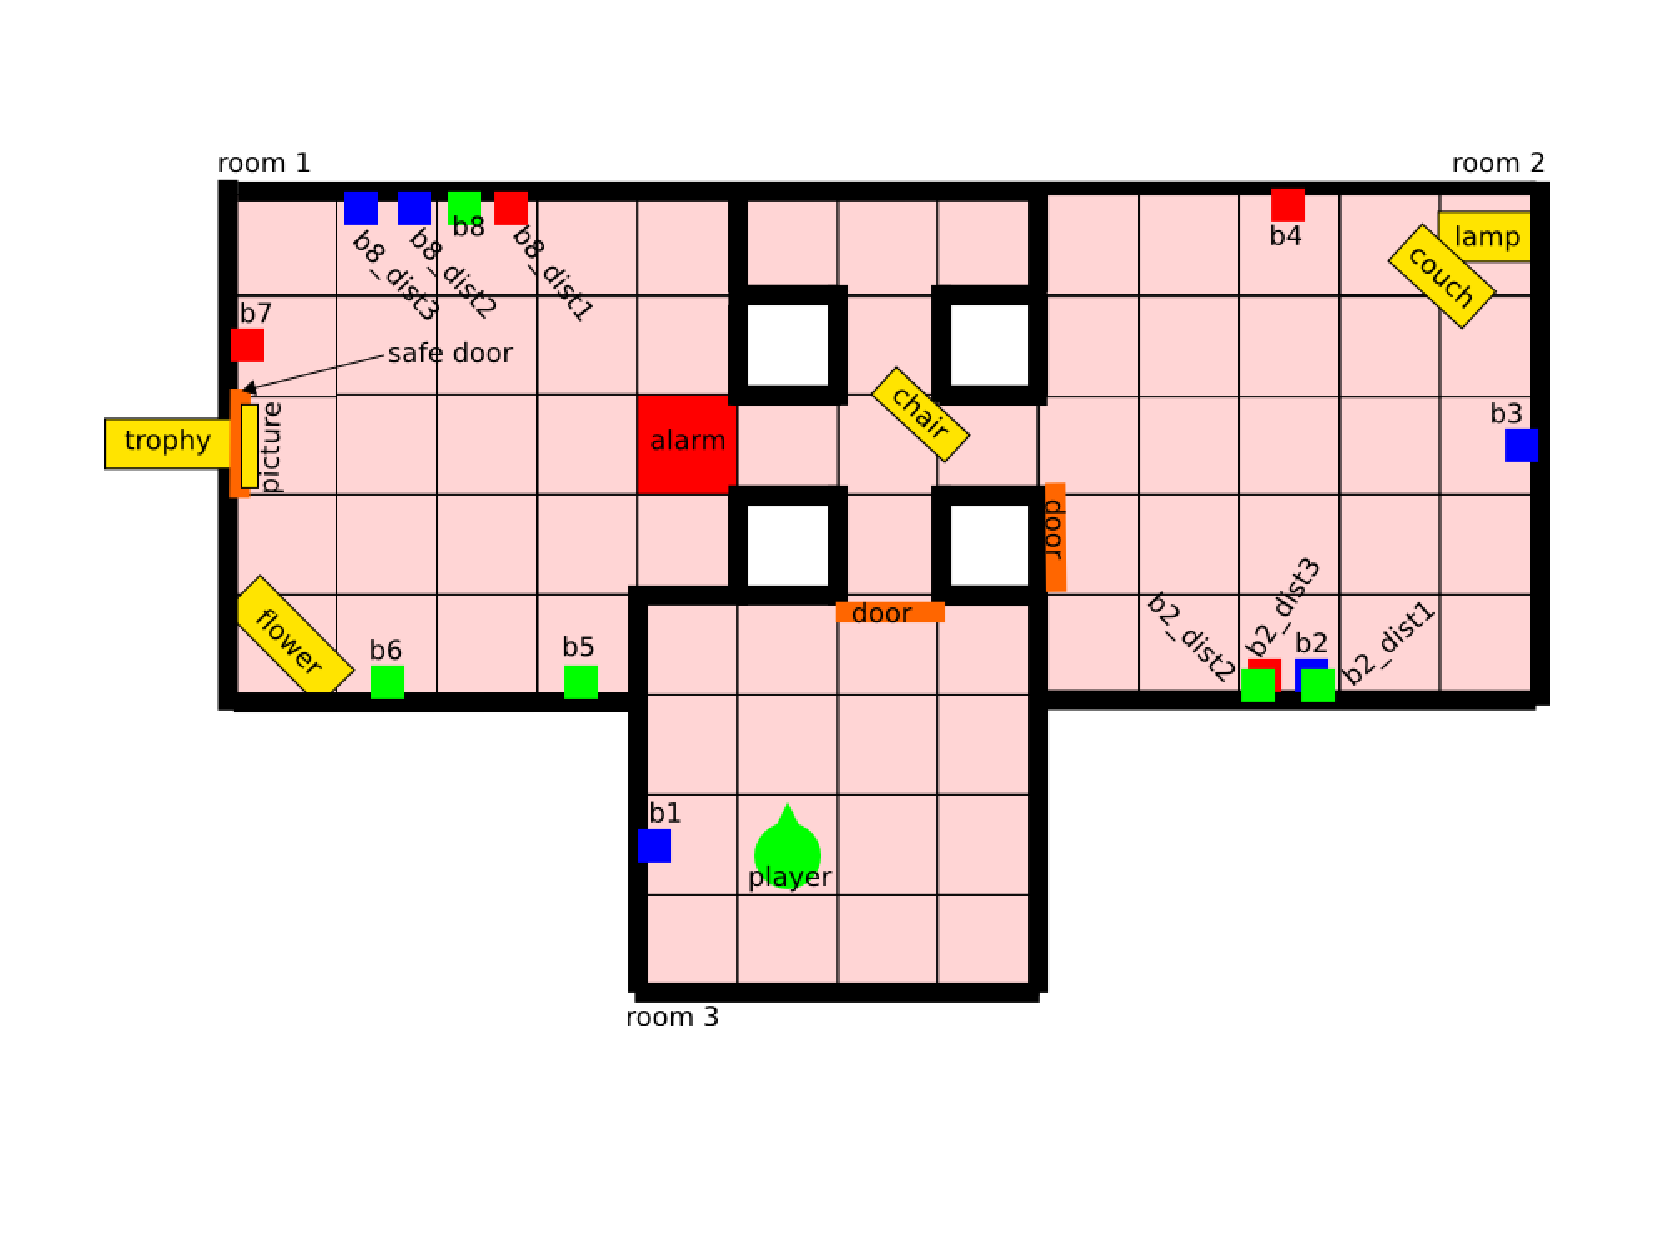
\includegraphics[width=1 \columnwidth]{give_world_no_expl}
\caption{Map of the GIVE development world.}
  \label{fig:give-development-world}
\end{figure}

\todo{explain world? -- yes, definitely}


One crucial component of a GIVE system is a planner which will compute
a domain plan that consists of the actions the user has to execute to
achieve the goal.  For these purposes, the virtual world is
discretized into a planning problem in which each object has a
symbolic position and orientation.  The first few action instances in
the example domain could be $turn-left(north,west)$, $move(pos-3-2,
pos-2-2, west)$, $manipulate-b_1-off-on(pos-2-2)$,
$turn-right(west,north)$, \todo{complete this} and so on.  Under the
current implementation of the planning problem, the shortest plan for
getting the player from the initial state to the goal (in which they
are holding the trophy) has 104 steps, most of which are ``move''
actions.  The bulk of the GIVE problem is therefore a variant of the
Gridworld problem, which also involves finding a route through a world
with discrete positions -- but with the need to press buttons in the
right order and with somewhat more complicated room shapes.

It is interesting to note that although the task of a GIVE NLG system
could be seen as mapping a domain plan to a sequence of NL
instructions, this mapping is not trivial.  It would be
\emph{possible} to express the last part of the above example plan as
``turn right; walk forward; walk forward; turn right; walk forward;
walk forward; turn left; walk forward'', but this is a very clumsy way
of phrasing the instruction ``turn around and walk through the door''
that will frustrate users and lead to bad evaluation results.  In
other words, it is important to aggregate multiple movement actions
into a single NL instruction.  On the other hand, it may be necessary
to generate instructions that don't correspond to domain actions.  For
instance, it will be necessary to find a correct referring expression
for $b_1$ in order to express the action
$manipulate-b_1-off-on(pos-2-2)$.  The interaction between referring
and instructing can go much deeper than that.  Imagine, for example,
that the user just entered the top right room, and we want to instruct
them to press $b_4$.  At that point in time, the user can see six
different buttons, and generating a single instruction of the form
``push X'' is difficult.  However, an instruction sequence like ``walk
forward; turn left; now press the button right in front of you'' will
be successful and natural.  Here the first two instructions do double
duty by preparing the simple referring expression ``the button right
in front of you'', which is only valid after the user's position and
orientation changed.  A generation system that is supposed to generate
such instruction sequences must be tightly integrated with the planner
in order to exploit the simultaneous effect of the first two
instructions on the world and on the communicative situation.

\todo{equivalent plans; plan recognition; real-time requirements}


%%% Local Variables: 
%%% mode: latex
%%% TeX-master: "experiences"
%%% End: 
